% Customizable fields and text areas start with % >> below.
% Lines starting with the comment character (%) are normally removed before release outside the collaboration, but not those comments ending lines

% svn info. These are modified by svn at checkout time.
% The last version of these macros found before the maketitle will be the one on the front page,
% so only the main file is tracked.
% Do not edit by hand!
\RCS$Revision: 464952 $
\RCS$HeadURL: svn+ssh://svn.cern.ch/reps/tdr2/papers/EXO-16-050/trunk/EXO-16-050.tex $
\RCS$Id: EXO-16-050.tex 464952 2018-06-18 09:24:35Z bmaier $
%%%%%%%%%%%%% local definitions %%%%%%%%%%%%%%%%%%%%%
% This allows for switching between one column and two column (cms@external) layouts
% The widths should  be modified for your particular figures. You'll need additional copies if you have more than one standard figure size.
\newlength\cmsFigWidth
\ifthenelse{\boolean{cms@external}}{\setlength\cmsFigWidth{0.85\columnwidth}}{\setlength\cmsFigWidth{0.4\textwidth}}
\ifthenelse{\boolean{cms@external}}{\providecommand{\cmsLeft}{top\xspace}}{\providecommand{\cmsLeft}{left\xspace}}
\ifthenelse{\boolean{cms@external}}{\providecommand{\cmsRight}{bottom\xspace}}{\providecommand{\cmsRight}{right\xspace}}


\renewcommand{\HGG}{\ensuremath{\Ph\rightarrow\gamma\gamma}\xspace}
\newcommand{\Hbb}{\ensuremath{\Ph\rightarrow\PQb\PAQb}\xspace}
\newcommand{\tt}{\ensuremath{\mathrm{t\bar{t}}}\xspace}
\newcommand{\bb}{\ensuremath{\PQb\PAQb}\xspace}
\newcommand{\mdm}{\ensuremath{m_{\chi}}\xspace}
\newcommand{\Nt}{\ensuremath{\mathrm{N}_{2}}\xspace}
\newcommand{\Ntd}{\ensuremath{\mathrm{N}_{2}^{DDT}}\xspace}
\newcommand{\msd}{\ensuremath{m_{SD}}\xspace}
\newcommand{\qq}{\ensuremath{\PQq\PAQq}\xspace}
\newcommand{\mzp}{\ensuremath{m_{\PZpr}}\xspace}
\renewcommand{\Az}{\ensuremath{\cmsSymbolFace{A}}\xspace}
\newcommand{\ptm}{\ensuremath{p_{\mathrm{T}}^{\text{miss}}}\xspace}
\renewcommand{\MET}{\ptm}
\renewcommand{\ETm}{\ptm}
\newcommand{\maz}{\ensuremath{m_{\Az}}\xspace}
\newcommand{\gzp}{\ensuremath{g_{\PZpr}}\xspace}
\newcommand{\MADGRAPHAMC} {\MADGRAPH{}5\_a\MCATNLO}
\newcommand{\x}{\ensuremath{\phantom{0}}}

%%%%%%%%%%%%%%%  Title page %%%%%%%%%%%%%%%%%%%%%%%%
\cmsNoteHeader{EXO-16-050} % This is over-written in the CMS environment: useful as preprint no. for export versions
% >> Title: please make sure that the non-TeX equivalent is in PDFTitle below
\title{Search for associated production of dark matter with a Higgs boson decaying to a pair of bottom quarks in $pp$ collisions at $sqrt(s)$ = 13 TeV}

% >> Authors
%Author is always "The CMS Collaboration" for PAS and papers, so author, etc, below will be ignored in those cases
%For multiple affiliations, create an address entry for the combination
%To mark authors as primary, use the \author* form

%\address[ncu]{National Central University}
%\address[fnal]{Fermilab}
%\address[cern]{CERN}
%\address[cern]{CERN}

\author[cern]{The CMS Collaboration}

% >> Date
% The date is in yyyy/mm/dd format. Today has been
% redefined to match, but if the date needs to be fixed, please write it in this fashion.
% For papers and PAS, \today is taken as the date the head file (this one) was last modified according to svn: see the RCS Id string above.
% For the final version it is best to "touch" the head file to make sure it has the latest date.
\date{\today}

% >> Abstract
% Abstract processing:
% 1. **DO NOT use \include or \input** to include the abstract: our abstract extractor will not search through other files than this one.
% 2. **DO NOT use %**                  to comment out sections of the abstract: the extractor will still grab those lines (and they won't be comments any longer!).
% 3. For PASs: **DO NOT use tex macros**         in the abstract: CDS MathJax processor used on the abstract doesn't understand them _and_ will only look within $$. The abstracts for papers are hand formatted so macros are okay.
\abstract{A search for dark matter produced in association with a Higgs boson decaying to a bottom quark-antiquark pair ($b\bar{b}$) is performed in
 proton-proton collisions at a center-of-mass energy of 13\TeV
 collected with the CMS detector at the LHC. The analyzed data sample corresponds to an integrated luminosity of $35.9\fbinv$. 
%Results are interpreted in the context of a $\mathrm{Z'}$-two-Higgs-doublet model, where a vector boson $\mathrm{Z'}$ is produced and decays into a Higgs boson and into two dark matter particles via  an intermediate heavy pseudoscalar particle, and in terms of the s-channel exchange of a vector mediator $\cPZpr_{B}$ that radiates a Higgs boson and decays into a dark matter particle pair.
The signal is characterized by a large missing transverse momentum recoiling against a $\text{b}\bar{\text{b}}$ system that has a large Lorentz boost. The number of events observed in the data is consistent with the standard model background prediction.  Results are interpreted in terms of limits on parameters in the 2HDM+a and baryonic Z' simplified models. For the baryonic Z' model, the presented results constitute the most stringent constraints to date. The 2HDM+a model is tested experimentally for the first time.
}
%In this model, the couplings of the $\cPZpr_{B}$ to 
%leptons are omitted. 
% and the Higgs sector is extended with four additional Higgs bosons.
%In this model, a high-mass resonance $\mathrm{Z'}$ decays into a pseudoscalar boson A and a light
%SM-like scalar Higgs boson, and the A decays to a pair of dark matter particles.
%No significant excesses are observed over the background prediction. Combining results from the two
%decay channels yields exclusion limits in the signal cross section in the $m_{\mathrm{Z'}}$- $m_{\textrm{A}}$ phase space.
%For example, the observed data exclude, for $\mathrm{Z'}$ coupling strength
%$g_{\mathrm{Z'}} = 0.8$,

% \abstract{A search for the dark matter is performed using events with large missing transverse momentum and a Higgs boson decaying into a pair of bottom quarks in a data sample of  proton-proton interactions at the centre-of-mass energy of 13 TeV collected with the CMS detector at the LHC in 2016. The data correspond to an integrated luminosity of 36 fb$^{-1}$. Results are interpreted in the framework of the Type-2 two-Higgs-doublet model and  baryonic-$\textrm{Z}^{'}$ model. Both of these models predict production of dark matter particle in association with the standard model Higgs boson. ... }

% >> PDF Metadata
% Do not comment out the following hypersetup lines (metadata). They will disappear in NODRAFT mode and are needed by CDS.
% Also: make sure that the values of the metadata items are sensible and are in plain text:
% (1) no TeX! -- for \sqrt{s} use sqrt(s) -- this will show with extra quote marks in the draft version but is okay).
% (2) no %.
% (3) No curly braces {}.
\hypersetup{%
pdfauthor={Raman Khurana, Benedikt Maier, Shin-Shan Eiko Yu, Matteo Cremonesi, Bo Jayatilaka},%
pdftitle={Search for dark matter in H(bb)+MET final state (full 2016 dataset)},%
pdfsubject={CMS},%
pdfkeywords={Dark matter, LHC, CMS, boosted Higgs boson tagging, physics, software, computing}}

\maketitle %maketitle comes after all the front information has been supplied
% >> Text
%%%%%%%%%%%%%%%%%%%%%%%%%%%%%%%%  Begin text %%%%%%%%%%%%%%%%%%%%%%%%%%%%%
%% **DO NOT REMOVE THE BIBLIOGRAPHY** which is located before the appendix.
%% You can take the text between here and the bibiliography as an example which you should replace with the actual text of your document.
%% If you include other TeX files, be sure to use "\input{filename}" rather than "\input filename".
%% The latter works for you, but our parser looks for the braces and will break when uploading the document.
%%%%%%%%%%%%%%%

%\section{Introduction}

Dark matter (DM) is one of the most compelling pieces of evidence for physics beyond the standard model (SM)~\cite{FNAL_Review}. Cosmological observations demonstrate that around 85\% of the mass of the Universe is comprised of DM. These observations make it highly likely that DM is composed primarily of weakly interacting massive particles (WIMPs). If non-gravitational interactions exist between DM and SM particles, DM could be produced by colliding SM particles at high energy. In many theories, the pair production of DM particles in hadron collisions proceeds through a spin-0 or spin-1 bosonic mediator, with the DM particles leaving the detector without a measurable signature. One way to observe them is when they are produced in association with a visible SM particle, which could be emitted directly from a quark as initial state radiation (ISR) or as part of new effective vertex couplings of DM to SM particles. 
Unlike that of Ws, Zs, jets, or photons, the ISR of the SM Higgs boson~\cite{HiggsObs_ATLAS, HiggsObs_CMS, HiggsObs_CMS_Long} is highly suppressed due to the Yukawa-like nature of its coupling strenght.

However, the associated production of a Higgs boson and DM particles, called the mono-H final state, can occur in a scheme where the Higgs boson is part of the interaction producing the DM particles, directly probing the structure of the effective DM-SM coupling.

We present a search for DM production in association with Higgs boson
decaying into a pair of bottom quark. As the H$\rightarrow \mathrm{b
  \bar{b}}$ decay channel has the largest branching ratio of any SM
Higgs boson decays it provides the largest potential signal yield. Results are presented for the full dataset of approximately 35.9~\fbinv collected by the CMS experiment at the CERN LHC at a center of mass energy of 13\TeV~in 2016. 


\section{Introduction} \label{intro}

Astrophysical evidence for dark matter (DM) is one of the most compelling motivations for
physics beyond the standard model
(SM)~\cite{dm1,dm2,dm3}. Cosmological observations demonstrate that
around 85\% of the matter in the universe is comprised of DM
\cite{planck} and are largely consistent with the hypothesis that DM is primarily composed of
weakly interacting massive particles (WIMPs). If nongravitational
interactions exist between DM and SM particles, DM could be produced
by colliding SM particles at high energy. Assuming the pair
production of DM particles in hadron collisions happens through a
spin-0 or spin-1 bosonic mediator coupled to the initial-state particles, the DM particles leave the
detector without a measurable signature. If DM particles are produced in association with a detectable SM particle, which could be emitted
as initial-state radiation (ISR) from the interacting constituents of the colliding protons, or through
new effective couplings between DM and SM particles, their
existence could be inferred via a large transverse momentum imbalance in the collision event. 


%Unlike in the case of W bosons, Z bosons, hadronic jets, or photons, 
While ISR production of the SM Higgs boson ($\Ph$)~\cite{HiggsObs_ATLAS, HiggsObs_CMS, HiggsObs_CMS_Long} is highly suppressed due to the Yukawa-like nature of its coupling strength to fermions, the associated production of a Higgs boson and DM particles
%,referred to as ``mono-h'' final state, 
can occur if the
Higgs boson takes part in the interaction producing the DM particles~\cite{monoHiggs3,2HDM,PhysRevD.89.075017}.
Such a production mechanism would allow to directly probe the structure of the effective DM-SM coupling.

In this paper, we  present a search for DM production in association
with an SM Higgs boson that decays into a bottom quark-antiquark pair ($\mathrm{b\bar{b}}$). As the $\Ph\rightarrow \mathrm{b\bar{b}}$ decay mode has the largest branching fraction of all Higgs boson decay modes allowed in the SM, it provides the largest signal yield. The search is performed using the data set collected by the CMS experiment~\cite{CMSdetector} at the CERN LHC at a center-of-mass energy of 13\TeV~in 2016, corresponding to an integrated luminosity of approximately 35.9\fbinv. 
Similar searches have been conducted at the LHC by both the ATLAS and the CMS Collaboration, analyzing data collected at 8~\cite{PhysRevLett.115.131801} and 13 TeV~\cite{PhysRevLett.119.181804,1807.02826}.
Results are interpreted in terms of two simplified models predicting this signature. The first one is type-2 two Higgs doublet model extended by an additional light pseudoscalar boson $a$ (2HDM+$a$)~\cite{Bauer2017}. The $a$ boson mixes with the scalar and pseudoscalar partners of the SM Higgs boson, and decays into a pair of DM particles,  $\chi\bar{\chi}$. The second model is a baryonic $\cPZpr$ model (baryonic Z')~\cite{PhysRevD.89.075017} where a vector mediator $\cPZpr$ is exchanged in the $s$-channel, radiates a Higgs boson, and subsequently decays into two DM 
particles. Representative Feynman diagrams for the two models are presented in Fig.~\ref{feyns}.


In the 2HDM+$a$ model, the DM particle candidate $\chi$ is a fermion that can couple to SM particles only through a spin-0, pseudoscalar mediator. Since the couplings of the new spin-0
mediator to SM gauge bosons are strongly suppressed, the 2HDM+$a$ model
is consistent with the measurements of the SM Higgs boson production and
decay modes, which so far show no significant deviation from SM predictions~\cite{Khachatryan:2016vau}. In contrast to previously explored 2HDM models~\cite{2HDM,Aaboud:2017yqz,Sirunyan:2017hnk}, the 2HDM+$a$ framework ensures gauge invariance and renormalizability. In this model, there are six mass eigenstates:
a light neutral charge-parity (CP)-even scalar \Ph, assumed to be the
observed 125\GeV Higgs boson, and a heavy neutral CP-even scalar \PH, that are the result of the mixing of the neutral CP-even weak eigenstates with the corresponding mixing angle $\alpha$;
a heavy neutral CP-odd pseudoscalar $A$ and a light neutral CP-odd pseudoscalar $a$, that are the result of the mixing of the CP-odd mediator $P$ with the CP-odd Higgs, with $\theta$ representing the associated mixing angle; and two heavy charged scalars \Hpm with identical mass. 

The masses of the two CP-odd Higgs bosons, the angle $\theta$ , and the ratio of vacuum
expectation values of the two CP-even Higgs bosons $\tan\beta$ are varied in this search. 
Perturbativity and unitarity put restrictions on the magnitudes and the
signs of the three quartic couplings
$\lambda_3,~\lambda_{\mathrm{P}1},~\lambda_{\mathrm{P}2}$,
and we therefore set their values to $\lambda_3=\lambda_{\mathrm{P}1}=\lambda_{\mathrm{P}2}=3$~\cite{Bauer2017}. The masses of the charged Higgs bosons and of the heavy CP-even Higgs boson are assumed to be the same as the mass of the heavy pseudoscalar, i.e., $m_{\PH}=m_{\Hpm}=m_{A}$. When an $m_{A}$ scan is performed, assumptions on $\tan\beta$ to be 1 and $\sin\theta$ to be 0.35 are made. The DM particle $\chi$ is assumed to have a mass of $m_\chi=10\GeV$.


The baryonic Z' model~\cite{PhysRevD.89.075017} is an extension of the SM with an additional U(1)$_{B}$ Z' gauge 
boson that couples to the baryon number $B$. The model predicts the existence of a new baryonic Dirac fermion that is neutral under SM gauge symmetries and stable due to the corresponding U(1)$_{B}$ symmetry. The state therefore serves as a good DM candidate.
To generate the  \cPZpr\ mass, a ``baryonic Higgs'' scalar is introduced to 
spontaneously break the U(1)$_B$ symmetry. Analogous to the SM, there remains 
a physical baryonic Higgs particle, h$_{B}$, with a coupling  $g_{\mathrm{h}_{B}\mathrm{Z'Z'}}$ to the Z' boson
and vacuum expectation value $v_{B}$. 
The \cPZpr\ and SM Higgs boson, h, interact with a coupling strength of 
$g_{\mathrm{h}_{B}\mathrm{Z'Z'}}$ = $m_{\cPZpr}^{2} \sin \theta/v_{B}$, where $\theta$ is the h-h$_{B}$ 
mixing angle. The chosen value for the \cPZpr\ coupling to quarks,
$g_\text{q}$, is 0.25 and the \cPZpr\ coupling to DM, $g_\chi$, is set to 1. This is well below the bounds $g_\text{q},g_\chi\sim4\pi$ where perturbativity and the validity of the effective field theory break down~\cite{PhysRevD.89.075017}. Constraints on the SM Higgs boson properties make the mixing angle $\theta$ consistent with $\cos\theta$ = 1 within order of 10\% uncertainties, thereby requiring  $\sin\theta$ to be less then 0.4~\cite{PhysRevD.89.075017}. In this search, $\theta$ is assumed to have $\sin\theta= 0.3$. It is also assumed that $g_{\text{h}\cPZpr\cPZpr}/m_{\mathrm{Z}'}=1$, which implies $v_B=m_{\cPZpr}\sin\theta$. This choice maximizes the cross section without violating the bounds imposed by SM measurements. The free parameters in the model under these assumptions are thus $m_{\cPZpr}$ and $m_\chi$, which are varied in this search.

\begin{figure}
\centering
 \subfloat{\includegraphics[width=0.4\textwidth]{figures/Feyn-2HDMa.pdf}}\hspace{1cm}
 \subfloat{\includegraphics[width=0.34\textwidth]{figures/Feyn-Baryonic.pdf}} \\
\caption{Feynman diagrams for the 2HDM+$a$ model (left) and the baryonic Z' model (right).}
\label{feyns}
\end{figure}


%The quantity \ptvecmiss, calculated as the negative vectorial sum of the transverse momentum (\pt) of all objects identified in an event, 
%represents the total
%momentum carried by the DM particles.
%The magnitude of this vector is referred to as \MET.
%For a given value of \mzp, the \pt of the \Az decreases as its mass increases.
%Therefore, the \MET spectrum softens with increasing \Az masses.
%A comparison of the \MET distributions expected from representative scenarios of the \cPZpr-2HDM model and the \cPZpr-Baryonic model are presented in Fig.~\ref{fig:met_signals}.


%\begin{figure}
%\centering
%\includegraphics[width=0.55\textwidth]{figures/puppimet_signals.pdf}
%\includegraphics[width=0.45\textwidth]{figures/ZpBaryonicModel.pdf}
%\caption{Reconstructed \MET for representative scenarios of two $\mathrm{h}+\mathrm{DM}$ models investigated. Coupling parameters are chosen as mentioned in the text. The \cPZpr-2HDM model in general has a significant harder \MET~spectrum than the \cPZpr-Baryonic model, which makes the former easier to distinguish from SM background processes.}
%\label{fig:met_signals}
%\end{figure}

Signal events are characterized by a large imbalance in the transverse
momentum (or hadronic recoil), which indicates the presence of invisible
DM particles, and by hadronic activity consistent with the production
of an SM Higgs boson that decays into a $\mathrm{b\bar{b}}$ pair. Thus, our search
strategy is to impose requirements on the mass of the reconstructed
Higgs boson candidate, together with the identification of the
products of hadronization of the two b quarks produced in the Higgs
boson decay, to define a data sample that is expected to be enriched
in signal events. Several different SM processes can mimic this topology, the most important of which are the top quark pair production and the production of a vector boson (V) in association with multiple jets. Statistically independent data samples are used to predict the hadronic recoil distribution for these SM processes that constitute the largest sources of background.
Both signal and background contributions to the data are extracted with a likelihood fit to the hadronic recoil distribution, performed simultaneously in all the different analysis subsamples.

%%===============================================================================
\section{The CMS detector, particle reconstruction, and event simulation}
\label{sec:cms}

The CMS detector, described in detail in Ref.~\cite{CMSdetector}, is a multipurpose apparatus designed to study high-transverse momentum ($\pt$) processes in proton-proton and heavy ion collisions.  
%
A superconducting solenoid occupies its central region, providing a magnetic field of 3.8\unit{T} parallel to the beam direction. 
%
Charged-particle trajectories are measured using the silicon pixel and strip trackers, which cover a pseudorapidity region of $\abs{\eta} < 2.5$. 
%
A lead tungstate (PbWO$_4$) crystal electromagnetic calorimeter (ECAL) and a brass/scintillator hadron calorimeter (HCAL) surround the tracking volume and cover $\abs{\eta} < 3$. 
%
The steel and quartz-fiber forward Cherenkov hadron calorimeter extends the coverage to $\abs{\eta} < 5$.  
%
The muon system consists of gas-ionization detectors embedded in the steel flux-return yoke outside the solenoid and covers $\abs{\eta} < 2.4$. 
%
The return yoke carries a 2\unit{T} return field from the solenoid.
%
%The first level of the CMS trigger system is designed to select events in less than 4\mus, using information from the calorimeters and muon detectors. 
Online event selection is accomplished via the two-tiered CMS trigger
system. The first level is designed to select events in less than
4\mus, using information
from the calorimeters and muon detectors. 
%
Subsequently, the high-level trigger-processor farm then reduces the event rate to several hundred Hz.
%


The particle-flow (PF) event algorithm~\cite{Sirunyan:2017ulk} aims at reconstructing and identifying each individual particle through an optimized combination of information from the different elements of the CMS detector. 
%
The energy of a photon is obtained directly from the ECAL measurement, corrected for effects from neglecting signals close to the detector noise level, termed zero-suppression in the following. 
%
The energy of an electron is determined from a combination of the electron momentum at the primary interaction vertex as determined by the tracker, the energy of the corresponding ECAL cluster, and the energy sum of all photons spatially compatible with originating from the electron track.
% 
The energy of a muon is obtained from the curvature of the corresponding track. 
%
The energy of a charged hadron is determined from a combination of its momentum measured in the tracker and the matching ECAL and HCAL energy deposits, corrected for zero-suppression effects and for the response function of the calorimeters to hadronic showers. 
%
Finally, the energy of a neutral hadron is obtained from the corresponding corrected ECAL and HCAL energy.
%

\section{Data and simulated samples}\label{sec:datasets}
%This analysis uses pp collision data at $\sqrt{s}=13\TeV$ recorded by the CMS experiment at the LHC during 2016.
%
%The data correspond to an integrated luminosity of $35.9\,\text{fb}^{-1}$. 
%
%Control regions obtained by requiring the presence of muons or electrons are employed in the search for $\MET+\mathrm{h}(\mathrm{b}\bar{\mathrm{b}})$; therefore, the \MET and SingleElectron datasets are used for offline analysis. 
%
%The \MET dataset includes muon pass-through triggers, which allow for selecting events with high $\MET$ or high muon recoil.


Signal samples are generated at leading order (LO) accuracy in quantum chromodynamics perturbation theory (QCD) using the \MADGRAPH{\textsc 5\_aMC@NLO}~\cite{amcatnlo} program.
%


To model the expectation from SM Higgs boson backgrounds as well as the \ttbar and single top quark backgrounds, the {\sc Powheg~v2}~\cite{Nason:2004rx,Frixione:2007vw,Alioli:2010xd} generator is used. All these processes are generated at the next-to-leading order (NLO) in QCD.
% 
Events with multiple jets produced through the strong interaction (referred to as QCD multijet events) are generated at LO using \MADGRAPH{\textsc 5\_aMC@NLO} v2.3.3.
%
Simulated samples of Z+jets and W+jets processes are generated at LO using \MADGRAPH{\textsc 5\_aMC@NLO} v2.3.3. Jets stemming from the matrix element calculations are matched to parton shower jets using the MLM prescription~\cite{mlm}.
%
The samples are corrected by weighting the \pt of the respective boson with NLO QCD corrections obtained from large samples of events generated with \MADGRAPH{\textsc 5\_aMC@NLO} and the FxFx merging technique~\cite{fxfx}.
%
The samples are further corrected by applying NLO electroweak corrections obtained from calculations~\cite{Kuhn:2005gv,Kallweit:2015fta,Kallweit:2015dum} that depend on boson \pt.
%
Predictions for the associated production of SM vector boson (i.e., diboson) production are obtained at LO with the {\sc Pythia 8.205}~\cite{Sjostrand:2014zea} generator.
%


For all the processes the LO or NLO the NNPDF30 parton distribution function~\cite{Ball:2014uwa} is used at LO or NLO. 
%
Parton showering, fragmentation, and hadronization are simulated with {\sc Pythia 8.2} using the CUETP8M1~\cite{ue1,ue2} tune. 
%
A {\sc Geant4}-based simulation of the CMS detector~\cite{geant4} is applied to all the simulated processes. 
%
Additional inelastic proton-proton interactions in the same or a neighboring bunch crossing (pileup) is included in the simulation.
%
The pileup distribution is corrected to match the corresponding distribution observed in data. 

\input{eventReco.tex}
The signal is characterized by high \MET, no isolated leptons, and a CA15 jet identified as a Higgs boson candidate. In the signal region (SR) described
below, the dominant background contributions arise from Z+jets, W+jets, and \ttbar production. To model these processes data events in different control regions (CR) are used: single-lepton CRs are designed to constrain the \ttbar and W +jets backgrounds, while dilepton CRs constrain the Z+jets background contribution. The hadronic recoil $U$ defined by removing the \pt of the lepton(s) from the \MET computation in CRs is used as proxy for the \MET distribution of the main background processes in SR. 

Events are selected online by requiring large \MET.
% (to be greater than thresholds of $90$, $100$, $110$, or $120\GeV$) and large $H_{\mathrm{T}}^{\mathrm{miss}}$. Online \MET is calculated as the magnitude of the negative vectorial sum of the \pt of all particles at the trigger level and $H_{\mathrm{T}}^{\mathrm{miss}}$ is defined as the magnitude of the vectorial sum of the \pt of all jets in the event with 
%$p_{\mathrm{T}}>20\GeV$. 
The identified muons are not used in the \MET calculation performed online.
Additional events selected by requiring high-\pt single electrons are used to populate the CRs. 
%Thresholds imposed online on the electron \pt vary from 25\,GeV to 105\,GeV depending on the identification and isolation criteria.  

Offline events are selected requiring \MET ($U$) to be larger than 200~\GeV in the SR (CRs). A single CA15 jet with \pt greater than 200~\GeV and $|\eta|<2.4$ is required as the Higgs boson candidate. Appropriate requirements on its mass and its $N_2$ are placed in order to identify it as a $\mathrm{H}\to\mathrm{b}\bar{\mathrm{b}}$-tagged jet.
 
Multijet events can act as a source of background when the energy of at least one of the jets is mismeasured. 
Therefore, the absolute difference between the azimuthal angles of the vector \ptvecmiss\ and any other AK4 jet with $\pt>30~\GeV$ 
is required to be $>0.4$\,rad. 

The event preselection described above is common for the SR and all the CRs. The preselected events are split into different SR and CRs based on their lepton multiplicity and the presence of a narrow b tagged AK4 jet non overlapping with the Higgs candidate CA15 jet.
% Table~\ref{tab:event_selection} summarizes the differents requirements that define the SR and the CRs. 

%\begin{table}
%  \begin{center}
%  \caption{Event selection used to separate SR and CRs. This selection is applied on top of the preselection common to all regions, 
%as described in the text. } \label{tab:event_selection}
%    \begin{tabular}{  l | c | c | c  }
%      \hline \hline
%        region   & additional AK4 b tag   & leptons & double-b tag \\ \hline
%        signal   & 0                & 0       & pass \\ \hline
%        \ttbar   & 1                & 1       & pass/fail\\ \hline
%        W        & 0                & 1       & pass/fail\\ \hline
%        Dilepton & 0                & 2       & pass/fail\\
%      \hline \hline
%    \end{tabular}
%  \end{center}
%\end{table}


For the SR, events are rejected if they have any isolated electrons (muons) with $\pt >10\GeV$ and $|\eta|< 2.5$ (2.4) or 
any $\tau_\mathrm{had}$ candidates with $\pt > 18$\GeV and $|\eta|<2.3$~\cite{Khachatryan:2015hwa,Chatrchyan:2013sba,CMSTauJINST}. The events are further required to have no good quality photon with $\pt> 15$\GeV and $|\eta|<2.5$. An additional requirement on double-b tagger output of the selected Higgs boson candidate CA15 jet is placed.
To reduce the contamination from top quark pair production, the events must not have any additional AK4 b-tagged jets or more than one additional AK4 jet.
Figure \ref{Fig_cr_Recoil_fail} shows the expected \MET distribution in the the SR for all the expected SM backgrounds with \cPZpr-2HDM model signal hypothesis overlaid on it. 

\begin{figure}
\centering
 \subfloat{\includegraphics[width=0.4\textwidth]{figures/dataMC/MSDcorr_stackedPostfit_signal.pdf}} 
 \subfloat{\includegraphics[width=0.4\textwidth]{figures/dataMC/MSDcorr_stackedPostfit_signal_masked.pdf}} \\
\caption{Shown is the \MET distribution in the signal region after a fit to data including the signal region (left) and excluding the signal region (right).}
\label{Fig_cr_Recoil_fail}
\end{figure}

%The different CRs defined in Table~\ref{tab:event_selection} are used to control the three main background processes.  Since the hadronic recoil $U$ is computed removing the muon(s) or the electron(s) from the \MET calculation, its distribution can be used as a proxy to model the \MET distribution in the SR. 
%Both the normalization and the shape of the \ttbar, Z+jets, and W+jets background processes are constrained by transfer factors from the CRs to the SR estimated in bins of $U$. These transfer factors correlate the same bins across all regions and are allowed to vary within uncertainties.% as described in Section~\ref{sec:systematics}.
To estimate the Z+jets production in the signal region, CRs enriched in dimuon and dielectron events are used.
Dimuon events are selected online employing the same \MET triggers that are used in the SR.
These events are required to have two opposite-charge muons (having a \pt greater than $20\GeV$ and $10\GeV$ for the leading and trailing muon, respectively), that form an invariant mass between 60\GeV and 120\GeV.
The leading muon also has to pass tight identification and isolation requirements.
%Events in the dimuon region must also pass almost all other selection requirements imposed on the events in the signal region, wherein $U$ is substituted for \ptmiss.
%In order to increase the number of events in the dimuon CR, the requirement of the fat jet b tag is not imposed.
Dielectron events are selected online using single electron triggers.%, which have a \pt threshold of $27\GeV$.
Two opposite-charge electrons with \pt greater than $10\GeV$ are required offline, and they must form an invariant mass between 60\GeV and 120\GeV.
To be on the plateau of the trigger efficiency, at least one of the two electrons must have $\pt>40\GeV$ and satisfy tight identification and isolation requirements.
%All selection criteria applied in the dimuon CR are applied in the dielectron CR.
Events that enter the signal selection due to the loss of a single lepton primarily arise from W+jets and semileptonic \ttbar events.
To estimate these backgrounds, four single-lepton samples are used: single muon and single electron, with or without an additional b-tagged AK4 jet.
The b-tagged single lepton CRs target \ttbar events, while the anti-b-tagged single lepton CRs target W+jets events.
Single muon events are selected using the \MET trigger.
The muon candidate in these events is required to have \pt greater than 20\GeV, and is required to be well identified and isolated.
%With the exception of b tagging, all other selection requirements used for signal events are imposed, using $U$ instead of \ptmiss.
In the b-tagged single muon CR, exactly one b-tagged AK4 jet non overlapping with the CA15 jet is required.
In the anti-b-tagged single muon CR, the b tagging requirement is reversed.
Each CR is split into two  subsamples depending on whether or
not they satisfy the same requirement on the output of double-b tagger imposed to define the SR. This allows for an {\it in situ} calibration of the scale factor that corrects the mis-identification probability of the double-b tagger for the three main backgrounds. 


The results are extracted with a binned liklihood fit (using the ROOStat package~\cite{roostats}) to the \MET and $U$ spectra. A simultaneous fit is performed on all the CRs and the SR. 
The dominant SM process in each CR is used to estimate at least one of the backgrounds in the SR. Each constraint is applied via a transfer factor $R$, which is ratio of the expected yield of the target process in the signal region and the expected yield of the process in the CR. $R$ is defined as a function of $U$ and estimated using simulation. 
If $b\ell$ is the subsample of the single lepton control sample that is used to estimate the \ttbar process in the SR, the free parameter $\mu^{\ttbar}_i$ will be included in the likelihood to represent the number of events observed in bin $i$ of $U$ in the SR. The expected number of events $N^{b\ell}_{i}$ is then given by $N^{b\ell}_{i}=  \dfrac{{\mu^{\ttbar}_{i}}}{R^{b\ell}_{i}}$.
The transfer factors $R^{\ell}$ and $R^{b\ell}$ used to constrain the W+jets and the $t\bar{t}$ background respectively are derived from simulation, taking into account the impact of lepton acceptances and efficiencies, the b-tagging efficiency, and, for the single electron control sample, the additional \MET requirement.
%This transfer factor explicitly includes hadronic tau leptons that fail the hadronic tau lepton identification criteria, which account for roughly 20-80\% of the total W+jets background in the high recoil region.  differences in \ptmiss trigger efficiencies observed between single-muon and dimuon events,
Because of a large \ttbar contamination in the W+jets pass CR, an additional transfer factor is imposed between the \ttbar in the b-tagged and anti-b-tagged single-lepton CRs.
%This allows for an estimation of the \ttbar contribution in the signal region to be made from W+jets CRs to be made from the b-tagged CR. 
A similar constraint is imposed to estimate the contamination from W+jets production in the $t\bar{t}$ CR composed by events that do not satisfy the requirement on the double-b output. 
The Z+jets background prediction in the signal region is connected to the dimuon and dielectron CRs through transfer factors ($R^{\ell\ell}$).
They are derived using simulation and account for the difference in the branching fractions of $\mathrm{Z}\rightarrow \nu\nu$~and $\mathrm{Z}\rightarrow \ell\ell$ decays and the impacts of lepton acceptances and selection efficiencies.


\section{Systematic uncertainties}

 Nuisance parameters are introduced into the likelihood fit to represent the systematic uncertainties of the search. They can either affect the rate or  the shape of \ptmiss ($U$) for a given process in the SR (CRs) and can be constrained in the fit. Shape uncertainties are incorporated by means of a Gaussian prior distribution, while rate uncertainties are given a log-normal prior distribution.

The \MET trigger efficiency is parametrized as a function of the
\MET. The uncertainty in its measurement is about 1\% and is included in the fit as a rate uncertainty.
The efficiencies of the single-electron triggers are parametrized as a
function of the electron \pt and an associated flat 1\% systematic uncertainty is added into the fit.

Uncertainties in the selection efficiencies amount to $1\%$ per selected muon or electron, while the uncertainty in the $\tau$ lepton veto is $3\%$; these rate uncertainties are correlated across all $U$ bins.

An uncertainty of $21\%$ in the heavy flavor fraction of
W+jets is reported in CMS measurements of inclusive W+jets
\cite{Khachatryan:2014uva} and W+heavy flavor
\cite{Khachatryan:2014uva,Chatrchyan:2013uza} production. Similarly, the uncertainty on the Z+heavy flavor fraction is measured to be $22\%$~\cite{Khachatryan:2014zya,Chatrchyan:2014dha}.
The magnitudes of the uncertainties in the W$/$Z+jets yields due to varying the heavy flavor components are different for each region (depending on the b tagging requirements) and range from $4\%$ to $5\%$ of the central W$/$Z+jets prediction. They are included as rate uncertainties and are correlated across all regions, but not correlated between the W+jets and Z+jets processes.
%
%These W+heavy flavor fraction uncertainties are correlated between all regions in the fit. 
%

The transfer factors $T$ are affected by uncertainties in the efficiencies of b-tagging or mistagging narrow isolated jets and by uncertainties related to lepton identification.  Differences on the order of 2\% in \MET trigger efficiencies observed between single-muon and dimuon events at lower $U$ values represent an additional systematic uncertainty in the transfer factors of the single-muon and dimuon CRs. All of these uncertainties can change the shape of the $U$ distribution. Shape uncertainties  due to higher order NLO or EW corrections, or PDF uncertainties, cancel out in the transfer factors when building the ratio of yields predicted in the SR and the corresponding CR due to the similarity of selection requirements between the SR and CRs.


\begin{table}\footnotesize
\begin{center}
  \caption{Systematic uncertainties, along with the type (rate/shape) of uncertainty and the affected processes. For the rate uncertainties, the percentage effect on the rate is quoted.}
\begin{tabular}{l r r}
  \hline\hline
Systematic uncertainty & Type & Processes \\
\hline
AK4 b tagging & shape & all \\
double-b tagging & shape & Z+jets, W+jets, \ttbar, SM h, signal\\
\ptmiss~trigger muon multiplicity & shape & Z+jets, W+jets \\
QCD scales & shape & SM h \\
PDF & shape & SM h \\
\ptmiss magnitude & 5\% & all \\
\ptmiss~trigger efficiency & 1\% & all \\
single-electron trigger & 1\% & all \\
lepton efficiency & 1\% per leg & all \\
$\tau$ lepton veto & 3\% & all \\
luminosity & 2.5\% & t, diboson, multijet, SM h, signal \\
CA15 jet energy & 4\% & t, diboson, multijet, SM h, signal \\
$N_2^\text{DDT}$ efficiency & 7\% & diboson, SM h, signal \\
theoretical cross section & 20\% & t, diboson\\
heavy flavor fraction & 4-5\% & Z+jets, W+jets\\
multijet normalization & 100\% & multijet \\
\hline\hline
  \end{tabular}
\label{tab:systs}
\end{center}
\end{table}





Two types of scale factors are used to correct for a potential difference in the double-b tagger misidentification efficiencies between data and prediction, one for W/Z+jets production and another for \ttbar production. Both factors affect only the overall rates of the respective processes, and they are measured directly in the fit by simultaneously fitting events that pass or fail the double-b tag requirement. The scale factors for W/Z+jets production are included in the fit as an unconstrained nuisance parameter. 
%
To take into account the variation of the double-b tagging efficiency
introduced by the uncertainty in the heavy flavor fraction of W/Z+jets
events, the efficiencies are reevaluated after varying the heavy
flavor component in the Monte Carlo simulation. The difference in the efficiency with respect to the nominal efficiency value is taken as a systematic uncertainty.
%
The values of the scale factor for \ttbar and its uncertainty are taken from an independent measurement in a statistically independent data sample. %In this case the efficiency is fixed, since no fluctuation is introduced by any effect like the varying heavy flavor fraction for W/Z+jets. 

%
%For W/Z+jets production, scale factors to correct the double-b tagger mis-identification efficiency are measured directly in the fit. This in-situ calibration is accomplished by performing the fit simultaneously with events that fail the double-b tagger requirement. The scale factor is included in the fit as an unconstrained nuisance. 
%
%To take into account the variation of the double-b tagger efficiency introduced by the uncertainty in the heavy flavor fraction of W/Z+jets events, up and down variation efficiencies are estimated. The difference between the up and down efficiency with respect to the central value is taken as a systematic uncertainty. 
%
%Additionally, a $U$-dependent shape uncertainty is put on the transfer factors tying the SR with the CRs that have an inverted requirement on the double-b tagger output; the uncertainties are 0\%, 2\%, 4\%, and 8\% for the four $U$ bins. It should be noted that the first bin is still allowed to vary due to the aforementioned scale factor that corrects the double-b pass/fail ratio globally.
%
%A similar approach is used for the measurement of the scale factor that corrects the mis-identification probability of \ttbar events. In this case the efficiency is fixed, since no fluctuation is introduced by any effect like the varying heavy flavor fraction for W/Z+jets.
%
In addition, a shape uncertainty that grows with \ptmiss or $U$ is applied on the transfer factors constraining the W/Z+jets backgrounds from the CRs with events that satisfy the inverted double-b tag criterion. This is done to account for potential effects with a residual \pt dependence. The shape uncertainty is anchored at the first bin where the magnitude of the uncertainty is 0\%, and increases to 8\% in the last hadronic recoil bin. 
%

A systematic uncertainty of $20\%$ is assigned to the single top quark background yields~\cite{Chatrchyan:1642680} and is correlated between the SR and the CRs. 
%
An uncertainty of $20\%$ is also assigned to the diboson production cross section~\cite{Khachatryan:2016txa,Khachatryan:2016tgp} and correlated across the SR and CRs.
%

Although an insignificant background, a conservative uncertainty of $100\%$ is used for the QCD multijet yield. 
%
This uncertainty is estimated using a sample enriched in multijet events. The sample is obtained by vetoing leptons and photons and by requiring $\ptmiss>250$\GeV and the minimum azimuthal angle between $\vec{p}_{\mathrm{T}}^{\mathrm{miss}}$ and the jet directions to be less than $0.1$\,rad.  The uncertainty is correlated between regions with the same
source of the faked object. That is, one nuisance parameter represents the
uncertainty in QCD multijet yields in the signal region and separate
nuisance parameters are introduced for the muon CRs and for electron CRs.
%

For processes estimated from Monte Carlo simulation, uncertainties in \ptmiss are obtained directly from simulation and propagated to $U$ following the standard CMS method~\cite{Khachatryan:2014gga}, which includes the jet energy correction uncertainties applied to the jets and \MET\ \cite{jec}. This results in a 4\% rate uncertainty in the backgrounds obtained from simulation due to the imperfect knowledge of the CA15 jet energy scale.
%
The \MET uncertainty amounts to a 5\% rate uncertainty that is included on each process in the final fit.
%

All processes for which a two-prong CA15 jet stemming from a resonance
decay is expected (the signal process, SM h production, diboson
production) contribute a 7\% rate uncertainty that is correlated
across all analysis regions. This corresponds to the uncertainty in
passing or failing the requirement on the substructure variable
$N_2^\text{DDT}$. The uncertainty has been derived in a control sample
enriched in \ttbar events, where the CA15 jet most often originates
from a hadronically decaying W boson that comes from the decay of one of the top quarks, but the corresponding b jet is out-of-cone. 
%
For the signal and the SM h processes, an uncertainty in the double-b tagging efficiency is applied that is 3\% for a CA15 jet with $\pt<350\GeV$, 4\% for the intermediate \pt~regime, and 8\% for $\pt>800$\GeV. These numbers have been derived through a measurement performed in a sample enriched in multijet events with double-muon-tagged $\text{g}\to\text{b}\bar{\text{b}}$ splittings. 
%

A systematic uncertainty of 2.5\% in the luminosity measurement~\cite{CMS-PAS-LUM-17-001} is included whenever the yields for a process in a specific bin are not determined from data. In these cases, appropriate QCD scale and PDF uncertainties are applied, too.
%

The impact of statistical uncertainties in predicted yields from simulation-driven backgrounds is negligible. However,  additional nuisance parameters corresponding to bin-by-bin statistical uncertainties on the transfer factors $T$ are considered. 
%

A summary of systematic uncertainties is presented in Table~\ref{tab:systs}.

Unlike the uncertainties described above, uncertainties on the signal predictions from QCD scale and PDF variations are not propagated as nuisance parameters. Instead, they are treated as uncertainties in the inclusive signal cross section. Due to the imperfect knowledge of PDFs at higher $x$, where $x$ is the momentum fraction carried by the partons participating in the hard interaction, the uncertainties increase with the mass of the final state and range from 4\% to 20\%.


\section{Results \label{sec:results}}

\begin{table}\footnotesize
\begin{center}
  \caption{Expected background event yields and observed numbers of events in data for $35.9\fbinv$. The expected number of signal events for 
the \cPZpr-2HDM model with \mz = 1000~\GeV (\maz = 300~\GeV), scaled to the nominal cross section, is also reported. 
}
\begin{tabular}{l r}
  \hline\hline
Process         & Yields          \\
\hline
Z+jets              &$ 303.9\pm6.8 $       \\
Single Top       &$29.2\pm2.2 $         \\
\ttbar          &$ 271.7\pm7.1 $        \\
W+jets          &$ 126.1\pm7.2 $            \\
SM H             &$ 29.0\pm0.2 $        \\
Diboson         &$ 27.0\pm3.1  $       \\
%Multijets       & ????  \\
\hline
Total background        &$ 786.7\pm12.8 $       \\
\hline \hline
\cPZpr-2HDM \mz = 1000~\GeV (\maz = 300~\GeV)        &$ 69.8\pm0.6 $       \\
%\cPZpr-2HDM \mz = 1700~\GeV (\maz = 300~\GeV)        &$ ????\pm ???? $     \\

%\cPZpr-Baryonic \mz = 100~\GeV (\mdm = 1~\GeV)        &$ ????\pm ???? $       \\
%\cPZpr-Baryonic \mz = 1000~\GeV(\mdm = 1~\GeV)        &$ ????\pm ???? $     \\
Data            & -         \\
\hline\hline
  \end{tabular}
\label{tab:eventYieldTable}
\end{center}
\end{table}



Table \ref{tab:eventYieldTable} shows the 
SR expected yields for each background and one signal mass hypothesis for the \cPZpr-2HDM model, along with the 
size of the statistical uncertainties.


Since no excess of events has been observed over the SM background expectation in the SR, the results of this search are interpreted in terms of an upper limit on the production cross 
section of DM candidates in association with a Higgs boson. 
The upper limits are calculated at 95\% confidence level (CL) using a modified frequentist method (CL$_s$) \cite{yellowReport, bib:CLS1, bib:CLS2} computed with an asymptotic approximation \cite{bib:CLS3}. 
A profile likelihood ratio is used as the test statistic in which systematic uncertainties are modeled as nuisance parameters.

\begin{figure}[htbp]
  \centering
  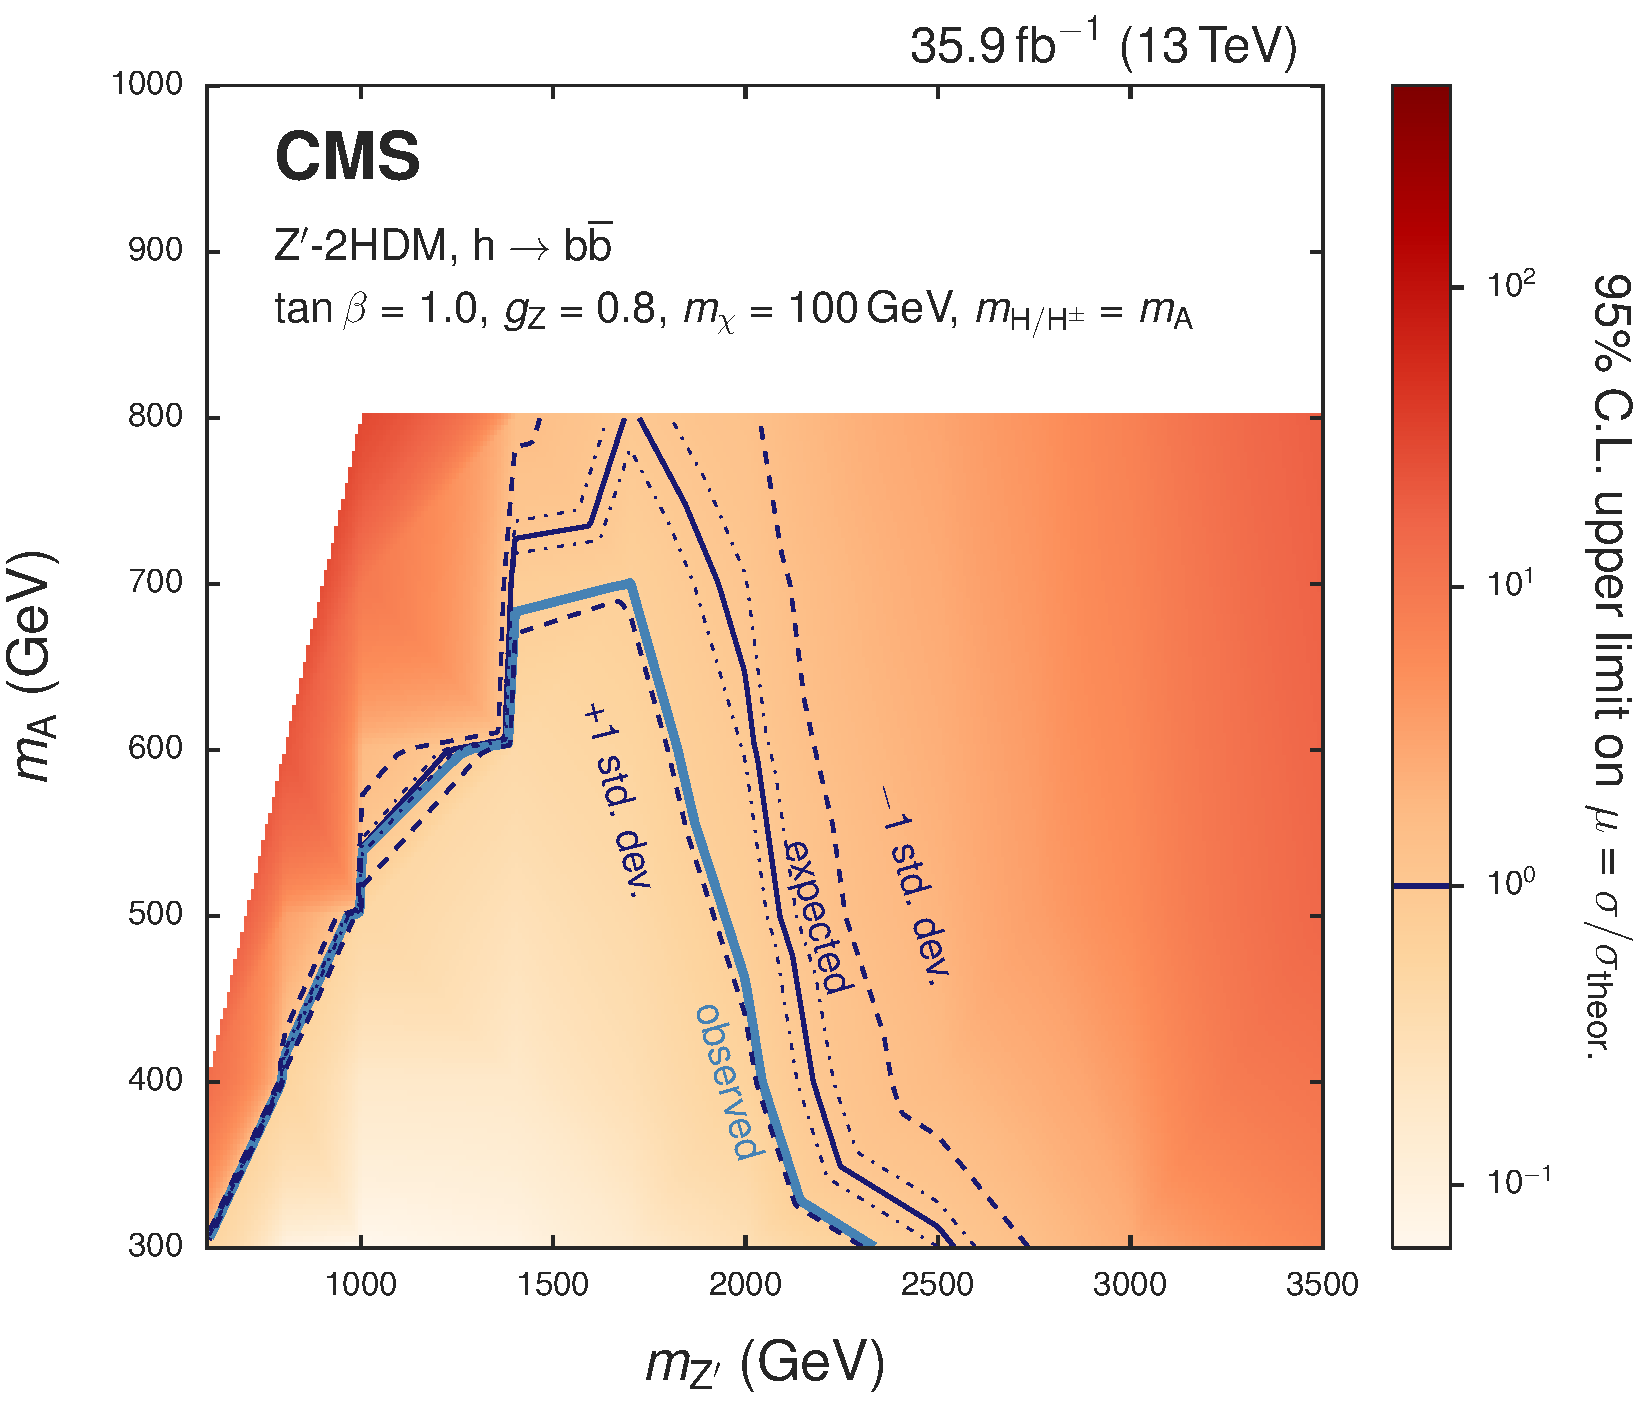
\includegraphics[width=0.475\textwidth]{figures/limits/limits_2hdm2d.png}
  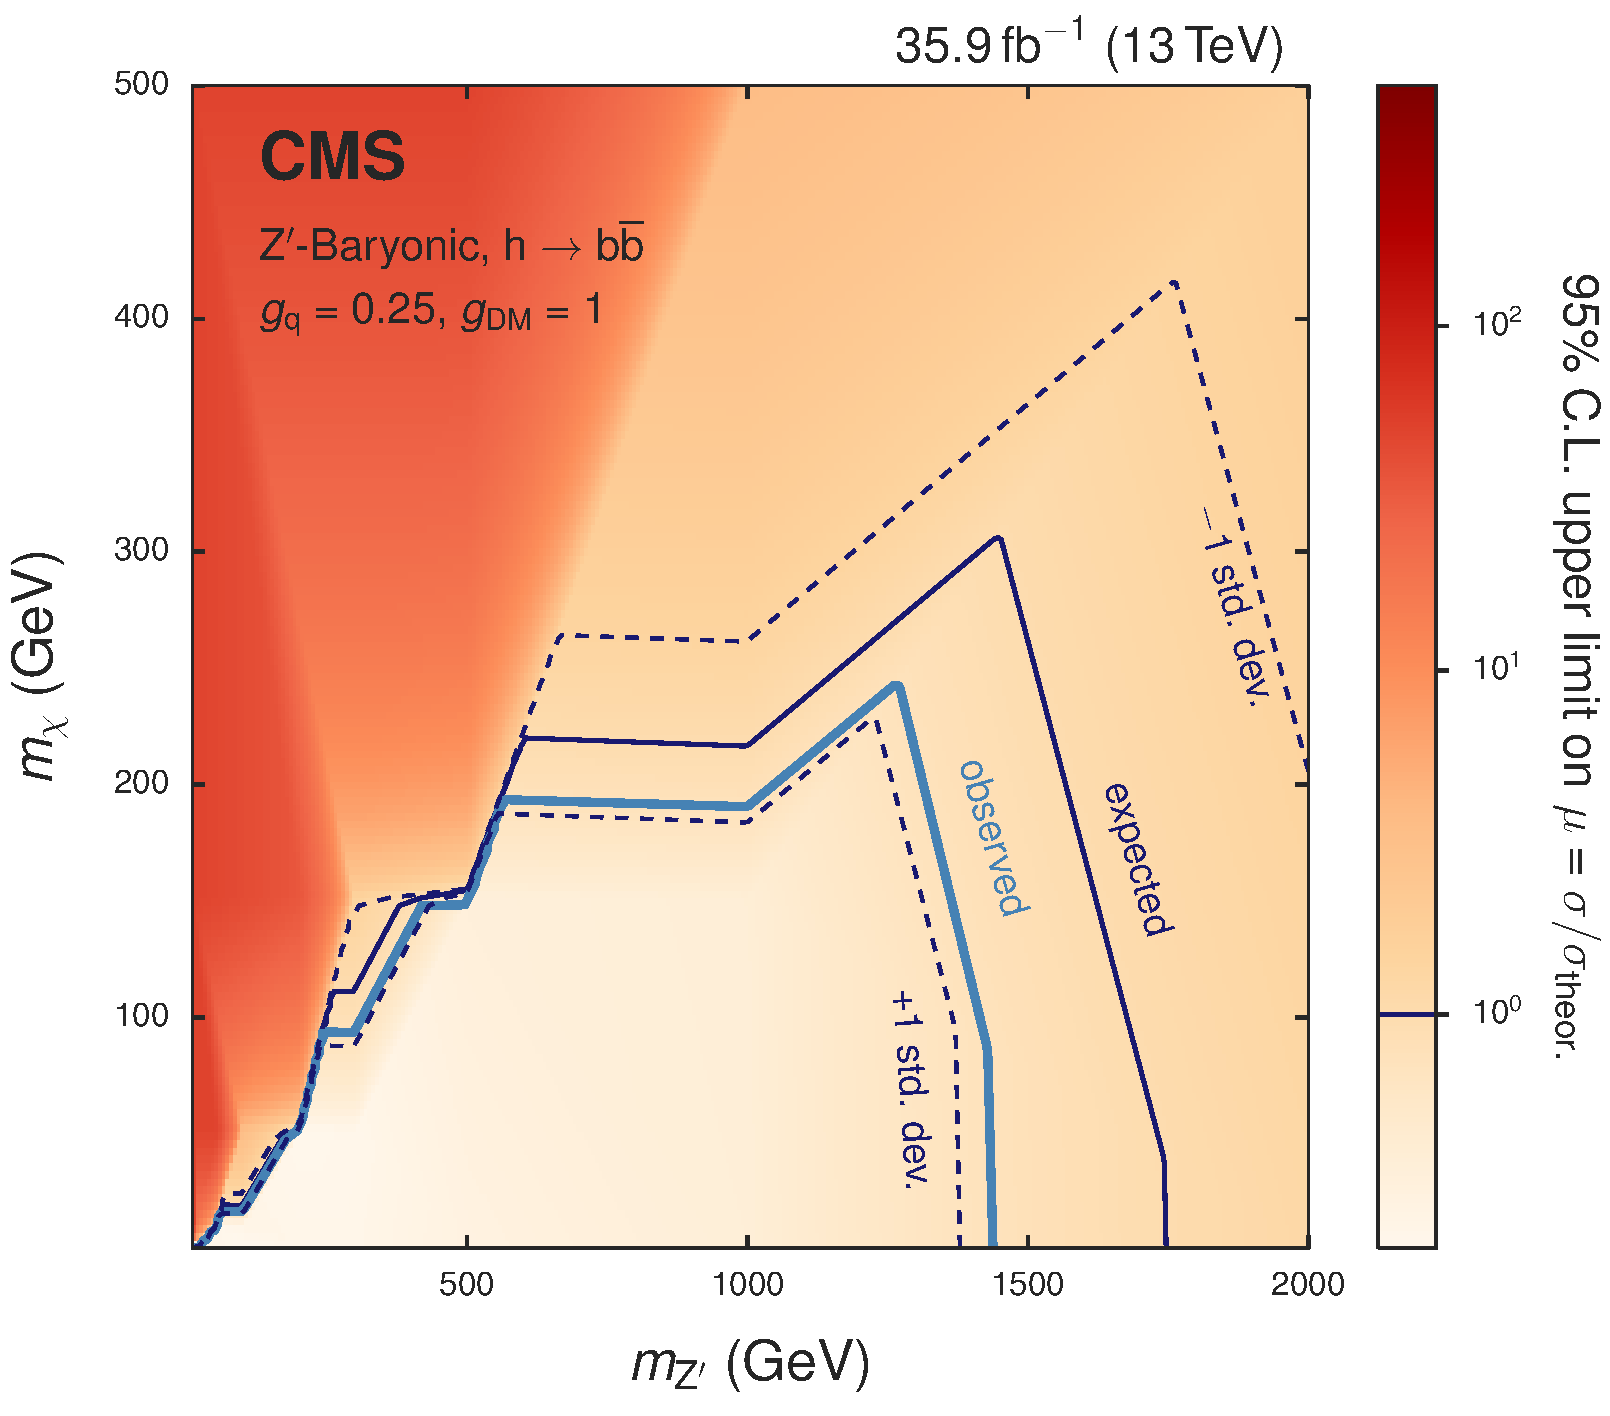
\includegraphics[width=0.475\textwidth]{figures/limits/limits_barzp2d.png}
  \caption{Upper limits on the signal strength modified for the 2HDM model (left) and Z'-Baryonic model (right).}
  \label{fig:limits}
\end{figure}

Figure~\ref{fig:limits} shows the expected and observed exclusions as a function of $m_{Z'}$ and $m_{A^0}$ for the \cPZpr-2HDM model and as a function of $m_{Z'}$ and $m_{\chi}$ for the 
baryonic $\cPZpr_{B}$ model. The excluded mass for $\mathrm{Z}'$ for $m_{A^0}=300$\,GeV is ???, while the largest excluded $\mathrm{Z}'$ mass in the $\mathrm{Z}'$-Baryonic model is ???. %Other assumptions are on $tan\beta = 1.0$, $g_{Z'} = 0.8$, and $m_{\chi} = 100$ GeV for the 2HDM, while for the Baryonic Z' model coupligs are assumed to be $g_{q} = 0.25, g_{\chi}=1~GeV$.

Results on the associated production of DM particles with Higgs boson decaying in a b-quark pair have been presented. Limits on the production cross section predicted by the \cPZpr-2HDM and the baryonic $\cPZpr_{B}$ model are set and they constitute the most stringent limits on the parameters in these models so far. 

%

Table \ref{tab:eventYieldTable} shows, for the \Hbb channel, the 
SR post-fit yields for each background and signal mass point along with the 
sum of the statistical and systematic uncertainties for the resolved and boosted regimes. 

For the \HGG channel, when applying the event selection to the data, two events are observed in the $m_{\gamma\gamma}$ sidebands and are used to 
evaluate the magnitude of the nonresonant background as described in Section~\ref{sec:bkg_model}. 
This yields an expected number of $0.38 \pm 0.27 (stat)$ nonresonant background events in the SR.
Expected resonant background contributions are taken from the simulation as detailed in Section~\ref{sec:bkg_model} and are $0.057 \pm 0.006 (stat)$ events considering both the Vh production (dominant) and the gluon fusion mode. Zero events are observed in the SR in the data.



Since no excess of events has been observed over the SM background expectation in the signal region, the results of this search are interpreted in terms of an upper limit on the production cross 
section of DM candidates in association with a Higgs boson via $\PZpr \rightarrow \Az \Ph \rightarrow \chi \bar{\chi} \PAQb\PQb(\gamma\gamma)$. 
The upper limits are computed at 95\% confidence level (CL) using a modified frequentist method (CL$_s$) \cite{yellowReport, bib:CLS1, bib:CLS2} computed with an asymptotic approximation \cite{bib:CLS3}. 
A profile likelihood ratio is used as the test statistic in which systematic uncertainties are modeled as nuisance parameters.
These limits are obtained as a function of \mzp and \maz for both Higgs boson decay channels and for the combination of the two. The two decay channels are combined using the branching ratios predicted by the SM.
In the combination of the two analyses, all signal and \MET-related systematic uncertainties as well as the systematic uncertainty on the integrated luminosity 
are assumed to be fully correlated.

Figure~\ref{fig:limitsexpected} (left) shows the 95\% CL expected and observed limits on the dark matter production cross section for 
\Hbb and \HGG for \maz = 300 GeV. 
Figures~\ref{fig:limitsexpected} (right) and~\ref{fig:limit2d} show the 95\% CL  expected and observed upper limits on the signal strength. 
For \maz = 300 GeV, the \mzp mass range 600 to 1780 \GeV is expected to be excluded with a 95\% CL when the signal model 
cross section is calculated using \gzp = 0.8. 
The observed data excludes, for \maz = 300 \GeV the \zp mass range of 600 to 1860 GeV. 
When the signal model cross section is calculated using the constrained \gzp, the expected exclusion range is 830 to 1890 GeV, 
and with the observed data the exclusion range is 770 to 2040 GeV. 



\begin{acknowledgments}
We congratulate our colleagues in the CERN accelerator departments for the excellent performance of the LHC and thank the technical and administrative staffs at CERN and at other CMS institutes for their contributions to the success of the CMS effort. In addition, we gratefully acknowledge the computing centers and personnel of the Worldwide LHC Computing Grid for delivering so effectively the computing infrastructure essential to our analyses. Finally, we acknowledge the enduring support for the construction and operation of the LHC and the CMS detector provided by the following funding agencies: BMWFW and FWF (Austria); FNRS and FWO (Belgium); CNPq, CAPES, FAPERJ, and FAPESP (Brazil); MES (Bulgaria); CERN; CAS, MoST, and NSFC (China); COLCIENCIAS (Colombia); MSES and CSF (Croatia); RPF (Cyprus); SENESCYT (Ecuador); MoER, ERC IUT, and ERDF (Estonia); Academy of Finland, MEC, and HIP (Finland); CEA and CNRS/IN2P3 (France); BMBF, DFG, and HGF (Germany); GSRT (Greece); OTKA and NIH (Hungary); DAE and DST (India); IPM (Iran); SFI (Ireland); INFN (Italy); MSIP and NRF (Republic of Korea); LAS (Lithuania); MOE and UM (Malaysia); BUAP, CINVESTAV, CONACYT, LNS, SEP, and UASLP-FAI (Mexico); MBIE (New Zealand); PAEC (Pakistan); MSHE and NSC (Poland); FCT (Portugal); JINR (Dubna); MON, RosAtom, RAS, RFBR and RAEP (Russia); MESTD (Serbia); SEIDI, CPAN, PCTI and FEDER (Spain); Swiss Funding Agencies (Switzerland); MST (Taipei); ThEPCenter, IPST, STAR, and NSTDA (Thailand); TUBITAK and TAEK (Turkey); NASU and SFFR (Ukraine); STFC (United Kingdom); DOE and NSF (USA).

\hyphenation{Rachada-pisek} Individuals have received support from the Marie-Curie program and the European Research Council and Horizon 2020 Grant, contract No. 675440 (European Union); the Leventis Foundation; the A. P. Sloan Foundation; the Alexander von Humboldt Foundation; the Belgian Federal Science Policy Office; the Fonds pour la Formation \`a la Recherche dans l'Industrie et dans l'Agriculture (FRIA-Belgium); the Agentschap voor Innovatie door Wetenschap en Technologie (IWT-Belgium); the Ministry of Education, Youth and Sports (MEYS) of the Czech Republic; the Council of Science and Industrial Research, India; the HOMING PLUS program of the Foundation for Polish Science, cofinanced from European Union, Regional Development Fund, the Mobility Plus program of the Ministry of Science and Higher Education, the National Science Center (Poland), contracts Harmonia 2014/14/M/ST2/00428, Opus 2014/13/B/ST2/02543, 2014/15/B/ST2/03998, and 2015/19/B/ST2/02861, Sonata-bis 2012/07/E/ST2/01406; the National Priorities Research Program by Qatar National Research Fund; the Programa Severo Ochoa del Principado de Asturias; the Thalis and Aristeia programs cofinanced by EU-ESF and the Greek NSRF; the Rachadapisek Sompot Fund for Postdoctoral Fellowship, Chulalongkorn University and the Chulalongkorn Academic into Its 2nd Century Project Advancement Project (Thailand); the Welch Foundation, contract C-1845; and the Weston Havens Foundation (USA).
\end{acknowledgments}


%\input{dataAndSimulation.tex}
%\input{eventReco.tex}
%The signal is characterized by high \MET, no isolated leptons, and a CA15 jet identified as a Higgs boson candidate. In the signal region (SR) described
below, the dominant background contributions arise from Z+jets, W+jets, and \ttbar production. To model these processes data events in different control regions (CR) are used: single-lepton CRs are designed to constrain the \ttbar and W +jets backgrounds, while dilepton CRs constrain the Z+jets background contribution. The hadronic recoil $U$ defined by removing the \pt of the lepton(s) from the \MET computation in CRs is used as proxy for the \MET distribution of the main background processes in SR. 

Events are selected online by requiring large \MET.
% (to be greater than thresholds of $90$, $100$, $110$, or $120\GeV$) and large $H_{\mathrm{T}}^{\mathrm{miss}}$. Online \MET is calculated as the magnitude of the negative vectorial sum of the \pt of all particles at the trigger level and $H_{\mathrm{T}}^{\mathrm{miss}}$ is defined as the magnitude of the vectorial sum of the \pt of all jets in the event with 
%$p_{\mathrm{T}}>20\GeV$. 
The identified muons are not used in the \MET calculation performed online.
Additional events selected by requiring high-\pt single electrons are used to populate the CRs. 
%Thresholds imposed online on the electron \pt vary from 25\,GeV to 105\,GeV depending on the identification and isolation criteria.  

Offline events are selected requiring \MET ($U$) to be larger than 200~\GeV in the SR (CRs). A single CA15 jet with \pt greater than 200~\GeV and $|\eta|<2.4$ is required as the Higgs boson candidate. Appropriate requirements on its mass and its $N_2$ are placed in order to identify it as a $\mathrm{H}\to\mathrm{b}\bar{\mathrm{b}}$-tagged jet.
 
Multijet events can act as a source of background when the energy of at least one of the jets is mismeasured. 
Therefore, the absolute difference between the azimuthal angles of the vector \ptvecmiss\ and any other AK4 jet with $\pt>30~\GeV$ 
is required to be $>0.4$\,rad. 

The event preselection described above is common for the SR and all the CRs. The preselected events are split into different SR and CRs based on their lepton multiplicity and the presence of a narrow b tagged AK4 jet non overlapping with the Higgs candidate CA15 jet.
% Table~\ref{tab:event_selection} summarizes the differents requirements that define the SR and the CRs. 

%\begin{table}
%  \begin{center}
%  \caption{Event selection used to separate SR and CRs. This selection is applied on top of the preselection common to all regions, 
%as described in the text. } \label{tab:event_selection}
%    \begin{tabular}{  l | c | c | c  }
%      \hline \hline
%        region   & additional AK4 b tag   & leptons & double-b tag \\ \hline
%        signal   & 0                & 0       & pass \\ \hline
%        \ttbar   & 1                & 1       & pass/fail\\ \hline
%        W        & 0                & 1       & pass/fail\\ \hline
%        Dilepton & 0                & 2       & pass/fail\\
%      \hline \hline
%    \end{tabular}
%  \end{center}
%\end{table}


For the SR, events are rejected if they have any isolated electrons (muons) with $\pt >10\GeV$ and $|\eta|< 2.5$ (2.4) or 
any $\tau_\mathrm{had}$ candidates with $\pt > 18$\GeV and $|\eta|<2.3$~\cite{Khachatryan:2015hwa,Chatrchyan:2013sba,CMSTauJINST}. The events are further required to have no good quality photon with $\pt> 15$\GeV and $|\eta|<2.5$. An additional requirement on double-b tagger output of the selected Higgs boson candidate CA15 jet is placed.
To reduce the contamination from top quark pair production, the events must not have any additional AK4 b-tagged jets or more than one additional AK4 jet.
Figure \ref{Fig_cr_Recoil_fail} shows the expected \MET distribution in the the SR for all the expected SM backgrounds with \cPZpr-2HDM model signal hypothesis overlaid on it. 

\begin{figure}
\centering
 \subfloat{\includegraphics[width=0.4\textwidth]{figures/dataMC/MSDcorr_stackedPostfit_signal.pdf}} 
 \subfloat{\includegraphics[width=0.4\textwidth]{figures/dataMC/MSDcorr_stackedPostfit_signal_masked.pdf}} \\
\caption{Shown is the \MET distribution in the signal region after a fit to data including the signal region (left) and excluding the signal region (right).}
\label{Fig_cr_Recoil_fail}
\end{figure}

%The different CRs defined in Table~\ref{tab:event_selection} are used to control the three main background processes.  Since the hadronic recoil $U$ is computed removing the muon(s) or the electron(s) from the \MET calculation, its distribution can be used as a proxy to model the \MET distribution in the SR. 
%Both the normalization and the shape of the \ttbar, Z+jets, and W+jets background processes are constrained by transfer factors from the CRs to the SR estimated in bins of $U$. These transfer factors correlate the same bins across all regions and are allowed to vary within uncertainties.% as described in Section~\ref{sec:systematics}.
To estimate the Z+jets production in the signal region, CRs enriched in dimuon and dielectron events are used.
Dimuon events are selected online employing the same \MET triggers that are used in the SR.
These events are required to have two opposite-charge muons (having a \pt greater than $20\GeV$ and $10\GeV$ for the leading and trailing muon, respectively), that form an invariant mass between 60\GeV and 120\GeV.
The leading muon also has to pass tight identification and isolation requirements.
%Events in the dimuon region must also pass almost all other selection requirements imposed on the events in the signal region, wherein $U$ is substituted for \ptmiss.
%In order to increase the number of events in the dimuon CR, the requirement of the fat jet b tag is not imposed.
Dielectron events are selected online using single electron triggers.%, which have a \pt threshold of $27\GeV$.
Two opposite-charge electrons with \pt greater than $10\GeV$ are required offline, and they must form an invariant mass between 60\GeV and 120\GeV.
To be on the plateau of the trigger efficiency, at least one of the two electrons must have $\pt>40\GeV$ and satisfy tight identification and isolation requirements.
%All selection criteria applied in the dimuon CR are applied in the dielectron CR.
Events that enter the signal selection due to the loss of a single lepton primarily arise from W+jets and semileptonic \ttbar events.
To estimate these backgrounds, four single-lepton samples are used: single muon and single electron, with or without an additional b-tagged AK4 jet.
The b-tagged single lepton CRs target \ttbar events, while the anti-b-tagged single lepton CRs target W+jets events.
Single muon events are selected using the \MET trigger.
The muon candidate in these events is required to have \pt greater than 20\GeV, and is required to be well identified and isolated.
%With the exception of b tagging, all other selection requirements used for signal events are imposed, using $U$ instead of \ptmiss.
In the b-tagged single muon CR, exactly one b-tagged AK4 jet non overlapping with the CA15 jet is required.
In the anti-b-tagged single muon CR, the b tagging requirement is reversed.
Each CR is split into two  subsamples depending on whether or
not they satisfy the same requirement on the output of double-b tagger imposed to define the SR. This allows for an {\it in situ} calibration of the scale factor that corrects the mis-identification probability of the double-b tagger for the three main backgrounds. 


The results are extracted with a binned liklihood fit (using the ROOStat package~\cite{roostats}) to the \MET and $U$ spectra. A simultaneous fit is performed on all the CRs and the SR. 
The dominant SM process in each CR is used to estimate at least one of the backgrounds in the SR. Each constraint is applied via a transfer factor $R$, which is ratio of the expected yield of the target process in the signal region and the expected yield of the process in the CR. $R$ is defined as a function of $U$ and estimated using simulation. 
If $b\ell$ is the subsample of the single lepton control sample that is used to estimate the \ttbar process in the SR, the free parameter $\mu^{\ttbar}_i$ will be included in the likelihood to represent the number of events observed in bin $i$ of $U$ in the SR. The expected number of events $N^{b\ell}_{i}$ is then given by $N^{b\ell}_{i}=  \dfrac{{\mu^{\ttbar}_{i}}}{R^{b\ell}_{i}}$.
The transfer factors $R^{\ell}$ and $R^{b\ell}$ used to constrain the W+jets and the $t\bar{t}$ background respectively are derived from simulation, taking into account the impact of lepton acceptances and efficiencies, the b-tagging efficiency, and, for the single electron control sample, the additional \MET requirement.
%This transfer factor explicitly includes hadronic tau leptons that fail the hadronic tau lepton identification criteria, which account for roughly 20-80\% of the total W+jets background in the high recoil region.  differences in \ptmiss trigger efficiencies observed between single-muon and dimuon events,
Because of a large \ttbar contamination in the W+jets pass CR, an additional transfer factor is imposed between the \ttbar in the b-tagged and anti-b-tagged single-lepton CRs.
%This allows for an estimation of the \ttbar contribution in the signal region to be made from W+jets CRs to be made from the b-tagged CR. 
A similar constraint is imposed to estimate the contamination from W+jets production in the $t\bar{t}$ CR composed by events that do not satisfy the requirement on the double-b output. 
The Z+jets background prediction in the signal region is connected to the dimuon and dielectron CRs through transfer factors ($R^{\ell\ell}$).
They are derived using simulation and account for the difference in the branching fractions of $\mathrm{Z}\rightarrow \nu\nu$~and $\mathrm{Z}\rightarrow \ell\ell$ decays and the impacts of lepton acceptances and selection efficiencies.


%\section{Systematic uncertainties}

 Nuisance parameters are introduced into the likelihood fit to represent the systematic uncertainties of the search. They can either affect the rate or  the shape of \ptmiss ($U$) for a given process in the SR (CRs) and can be constrained in the fit. Shape uncertainties are incorporated by means of a Gaussian prior distribution, while rate uncertainties are given a log-normal prior distribution.

The \MET trigger efficiency is parametrized as a function of the
\MET. The uncertainty in its measurement is about 1\% and is included in the fit as a rate uncertainty.
The efficiencies of the single-electron triggers are parametrized as a
function of the electron \pt and an associated flat 1\% systematic uncertainty is added into the fit.

Uncertainties in the selection efficiencies amount to $1\%$ per selected muon or electron, while the uncertainty in the $\tau$ lepton veto is $3\%$; these rate uncertainties are correlated across all $U$ bins.

An uncertainty of $21\%$ in the heavy flavor fraction of
W+jets is reported in CMS measurements of inclusive W+jets
\cite{Khachatryan:2014uva} and W+heavy flavor
\cite{Khachatryan:2014uva,Chatrchyan:2013uza} production. Similarly, the uncertainty on the Z+heavy flavor fraction is measured to be $22\%$~\cite{Khachatryan:2014zya,Chatrchyan:2014dha}.
The magnitudes of the uncertainties in the W$/$Z+jets yields due to varying the heavy flavor components are different for each region (depending on the b tagging requirements) and range from $4\%$ to $5\%$ of the central W$/$Z+jets prediction. They are included as rate uncertainties and are correlated across all regions, but not correlated between the W+jets and Z+jets processes.
%
%These W+heavy flavor fraction uncertainties are correlated between all regions in the fit. 
%

The transfer factors $T$ are affected by uncertainties in the efficiencies of b-tagging or mistagging narrow isolated jets and by uncertainties related to lepton identification.  Differences on the order of 2\% in \MET trigger efficiencies observed between single-muon and dimuon events at lower $U$ values represent an additional systematic uncertainty in the transfer factors of the single-muon and dimuon CRs. All of these uncertainties can change the shape of the $U$ distribution. Shape uncertainties  due to higher order NLO or EW corrections, or PDF uncertainties, cancel out in the transfer factors when building the ratio of yields predicted in the SR and the corresponding CR due to the similarity of selection requirements between the SR and CRs.


\begin{table}\footnotesize
\begin{center}
  \caption{Systematic uncertainties, along with the type (rate/shape) of uncertainty and the affected processes. For the rate uncertainties, the percentage effect on the rate is quoted.}
\begin{tabular}{l r r}
  \hline\hline
Systematic uncertainty & Type & Processes \\
\hline
AK4 b tagging & shape & all \\
double-b tagging & shape & Z+jets, W+jets, \ttbar, SM h, signal\\
\ptmiss~trigger muon multiplicity & shape & Z+jets, W+jets \\
QCD scales & shape & SM h \\
PDF & shape & SM h \\
\ptmiss magnitude & 5\% & all \\
\ptmiss~trigger efficiency & 1\% & all \\
single-electron trigger & 1\% & all \\
lepton efficiency & 1\% per leg & all \\
$\tau$ lepton veto & 3\% & all \\
luminosity & 2.5\% & t, diboson, multijet, SM h, signal \\
CA15 jet energy & 4\% & t, diboson, multijet, SM h, signal \\
$N_2^\text{DDT}$ efficiency & 7\% & diboson, SM h, signal \\
theoretical cross section & 20\% & t, diboson\\
heavy flavor fraction & 4-5\% & Z+jets, W+jets\\
multijet normalization & 100\% & multijet \\
\hline\hline
  \end{tabular}
\label{tab:systs}
\end{center}
\end{table}





Two types of scale factors are used to correct for a potential difference in the double-b tagger misidentification efficiencies between data and prediction, one for W/Z+jets production and another for \ttbar production. Both factors affect only the overall rates of the respective processes, and they are measured directly in the fit by simultaneously fitting events that pass or fail the double-b tag requirement. The scale factors for W/Z+jets production are included in the fit as an unconstrained nuisance parameter. 
%
To take into account the variation of the double-b tagging efficiency
introduced by the uncertainty in the heavy flavor fraction of W/Z+jets
events, the efficiencies are reevaluated after varying the heavy
flavor component in the Monte Carlo simulation. The difference in the efficiency with respect to the nominal efficiency value is taken as a systematic uncertainty.
%
The values of the scale factor for \ttbar and its uncertainty are taken from an independent measurement in a statistically independent data sample. %In this case the efficiency is fixed, since no fluctuation is introduced by any effect like the varying heavy flavor fraction for W/Z+jets. 

%
%For W/Z+jets production, scale factors to correct the double-b tagger mis-identification efficiency are measured directly in the fit. This in-situ calibration is accomplished by performing the fit simultaneously with events that fail the double-b tagger requirement. The scale factor is included in the fit as an unconstrained nuisance. 
%
%To take into account the variation of the double-b tagger efficiency introduced by the uncertainty in the heavy flavor fraction of W/Z+jets events, up and down variation efficiencies are estimated. The difference between the up and down efficiency with respect to the central value is taken as a systematic uncertainty. 
%
%Additionally, a $U$-dependent shape uncertainty is put on the transfer factors tying the SR with the CRs that have an inverted requirement on the double-b tagger output; the uncertainties are 0\%, 2\%, 4\%, and 8\% for the four $U$ bins. It should be noted that the first bin is still allowed to vary due to the aforementioned scale factor that corrects the double-b pass/fail ratio globally.
%
%A similar approach is used for the measurement of the scale factor that corrects the mis-identification probability of \ttbar events. In this case the efficiency is fixed, since no fluctuation is introduced by any effect like the varying heavy flavor fraction for W/Z+jets.
%
In addition, a shape uncertainty that grows with \ptmiss or $U$ is applied on the transfer factors constraining the W/Z+jets backgrounds from the CRs with events that satisfy the inverted double-b tag criterion. This is done to account for potential effects with a residual \pt dependence. The shape uncertainty is anchored at the first bin where the magnitude of the uncertainty is 0\%, and increases to 8\% in the last hadronic recoil bin. 
%

A systematic uncertainty of $20\%$ is assigned to the single top quark background yields~\cite{Chatrchyan:1642680} and is correlated between the SR and the CRs. 
%
An uncertainty of $20\%$ is also assigned to the diboson production cross section~\cite{Khachatryan:2016txa,Khachatryan:2016tgp} and correlated across the SR and CRs.
%

Although an insignificant background, a conservative uncertainty of $100\%$ is used for the QCD multijet yield. 
%
This uncertainty is estimated using a sample enriched in multijet events. The sample is obtained by vetoing leptons and photons and by requiring $\ptmiss>250$\GeV and the minimum azimuthal angle between $\vec{p}_{\mathrm{T}}^{\mathrm{miss}}$ and the jet directions to be less than $0.1$\,rad.  The uncertainty is correlated between regions with the same
source of the faked object. That is, one nuisance parameter represents the
uncertainty in QCD multijet yields in the signal region and separate
nuisance parameters are introduced for the muon CRs and for electron CRs.
%

For processes estimated from Monte Carlo simulation, uncertainties in \ptmiss are obtained directly from simulation and propagated to $U$ following the standard CMS method~\cite{Khachatryan:2014gga}, which includes the jet energy correction uncertainties applied to the jets and \MET\ \cite{jec}. This results in a 4\% rate uncertainty in the backgrounds obtained from simulation due to the imperfect knowledge of the CA15 jet energy scale.
%
The \MET uncertainty amounts to a 5\% rate uncertainty that is included on each process in the final fit.
%

All processes for which a two-prong CA15 jet stemming from a resonance
decay is expected (the signal process, SM h production, diboson
production) contribute a 7\% rate uncertainty that is correlated
across all analysis regions. This corresponds to the uncertainty in
passing or failing the requirement on the substructure variable
$N_2^\text{DDT}$. The uncertainty has been derived in a control sample
enriched in \ttbar events, where the CA15 jet most often originates
from a hadronically decaying W boson that comes from the decay of one of the top quarks, but the corresponding b jet is out-of-cone. 
%
For the signal and the SM h processes, an uncertainty in the double-b tagging efficiency is applied that is 3\% for a CA15 jet with $\pt<350\GeV$, 4\% for the intermediate \pt~regime, and 8\% for $\pt>800$\GeV. These numbers have been derived through a measurement performed in a sample enriched in multijet events with double-muon-tagged $\text{g}\to\text{b}\bar{\text{b}}$ splittings. 
%

A systematic uncertainty of 2.5\% in the luminosity measurement~\cite{CMS-PAS-LUM-17-001} is included whenever the yields for a process in a specific bin are not determined from data. In these cases, appropriate QCD scale and PDF uncertainties are applied, too.
%

The impact of statistical uncertainties in predicted yields from simulation-driven backgrounds is negligible. However,  additional nuisance parameters corresponding to bin-by-bin statistical uncertainties on the transfer factors $T$ are considered. 
%

A summary of systematic uncertainties is presented in Table~\ref{tab:systs}.

Unlike the uncertainties described above, uncertainties on the signal predictions from QCD scale and PDF variations are not propagated as nuisance parameters. Instead, they are treated as uncertainties in the inclusive signal cross section. Due to the imperfect knowledge of PDFs at higher $x$, where $x$ is the momentum fraction carried by the partons participating in the hard interaction, the uncertainties increase with the mass of the final state and range from 4\% to 20\%.


%\section{Results \label{sec:results}}

\begin{table}\footnotesize
\begin{center}
  \caption{Expected background event yields and observed numbers of events in data for $35.9\fbinv$. The expected number of signal events for 
the \cPZpr-2HDM model with \mz = 1000~\GeV (\maz = 300~\GeV), scaled to the nominal cross section, is also reported. 
}
\begin{tabular}{l r}
  \hline\hline
Process         & Yields          \\
\hline
Z+jets              &$ 303.9\pm6.8 $       \\
Single Top       &$29.2\pm2.2 $         \\
\ttbar          &$ 271.7\pm7.1 $        \\
W+jets          &$ 126.1\pm7.2 $            \\
SM H             &$ 29.0\pm0.2 $        \\
Diboson         &$ 27.0\pm3.1  $       \\
%Multijets       & ????  \\
\hline
Total background        &$ 786.7\pm12.8 $       \\
\hline \hline
\cPZpr-2HDM \mz = 1000~\GeV (\maz = 300~\GeV)        &$ 69.8\pm0.6 $       \\
%\cPZpr-2HDM \mz = 1700~\GeV (\maz = 300~\GeV)        &$ ????\pm ???? $     \\

%\cPZpr-Baryonic \mz = 100~\GeV (\mdm = 1~\GeV)        &$ ????\pm ???? $       \\
%\cPZpr-Baryonic \mz = 1000~\GeV(\mdm = 1~\GeV)        &$ ????\pm ???? $     \\
Data            & -         \\
\hline\hline
  \end{tabular}
\label{tab:eventYieldTable}
\end{center}
\end{table}



Table \ref{tab:eventYieldTable} shows the 
SR expected yields for each background and one signal mass hypothesis for the \cPZpr-2HDM model, along with the 
size of the statistical uncertainties.


Since no excess of events has been observed over the SM background expectation in the SR, the results of this search are interpreted in terms of an upper limit on the production cross 
section of DM candidates in association with a Higgs boson. 
The upper limits are calculated at 95\% confidence level (CL) using a modified frequentist method (CL$_s$) \cite{yellowReport, bib:CLS1, bib:CLS2} computed with an asymptotic approximation \cite{bib:CLS3}. 
A profile likelihood ratio is used as the test statistic in which systematic uncertainties are modeled as nuisance parameters.

\begin{figure}[htbp]
  \centering
  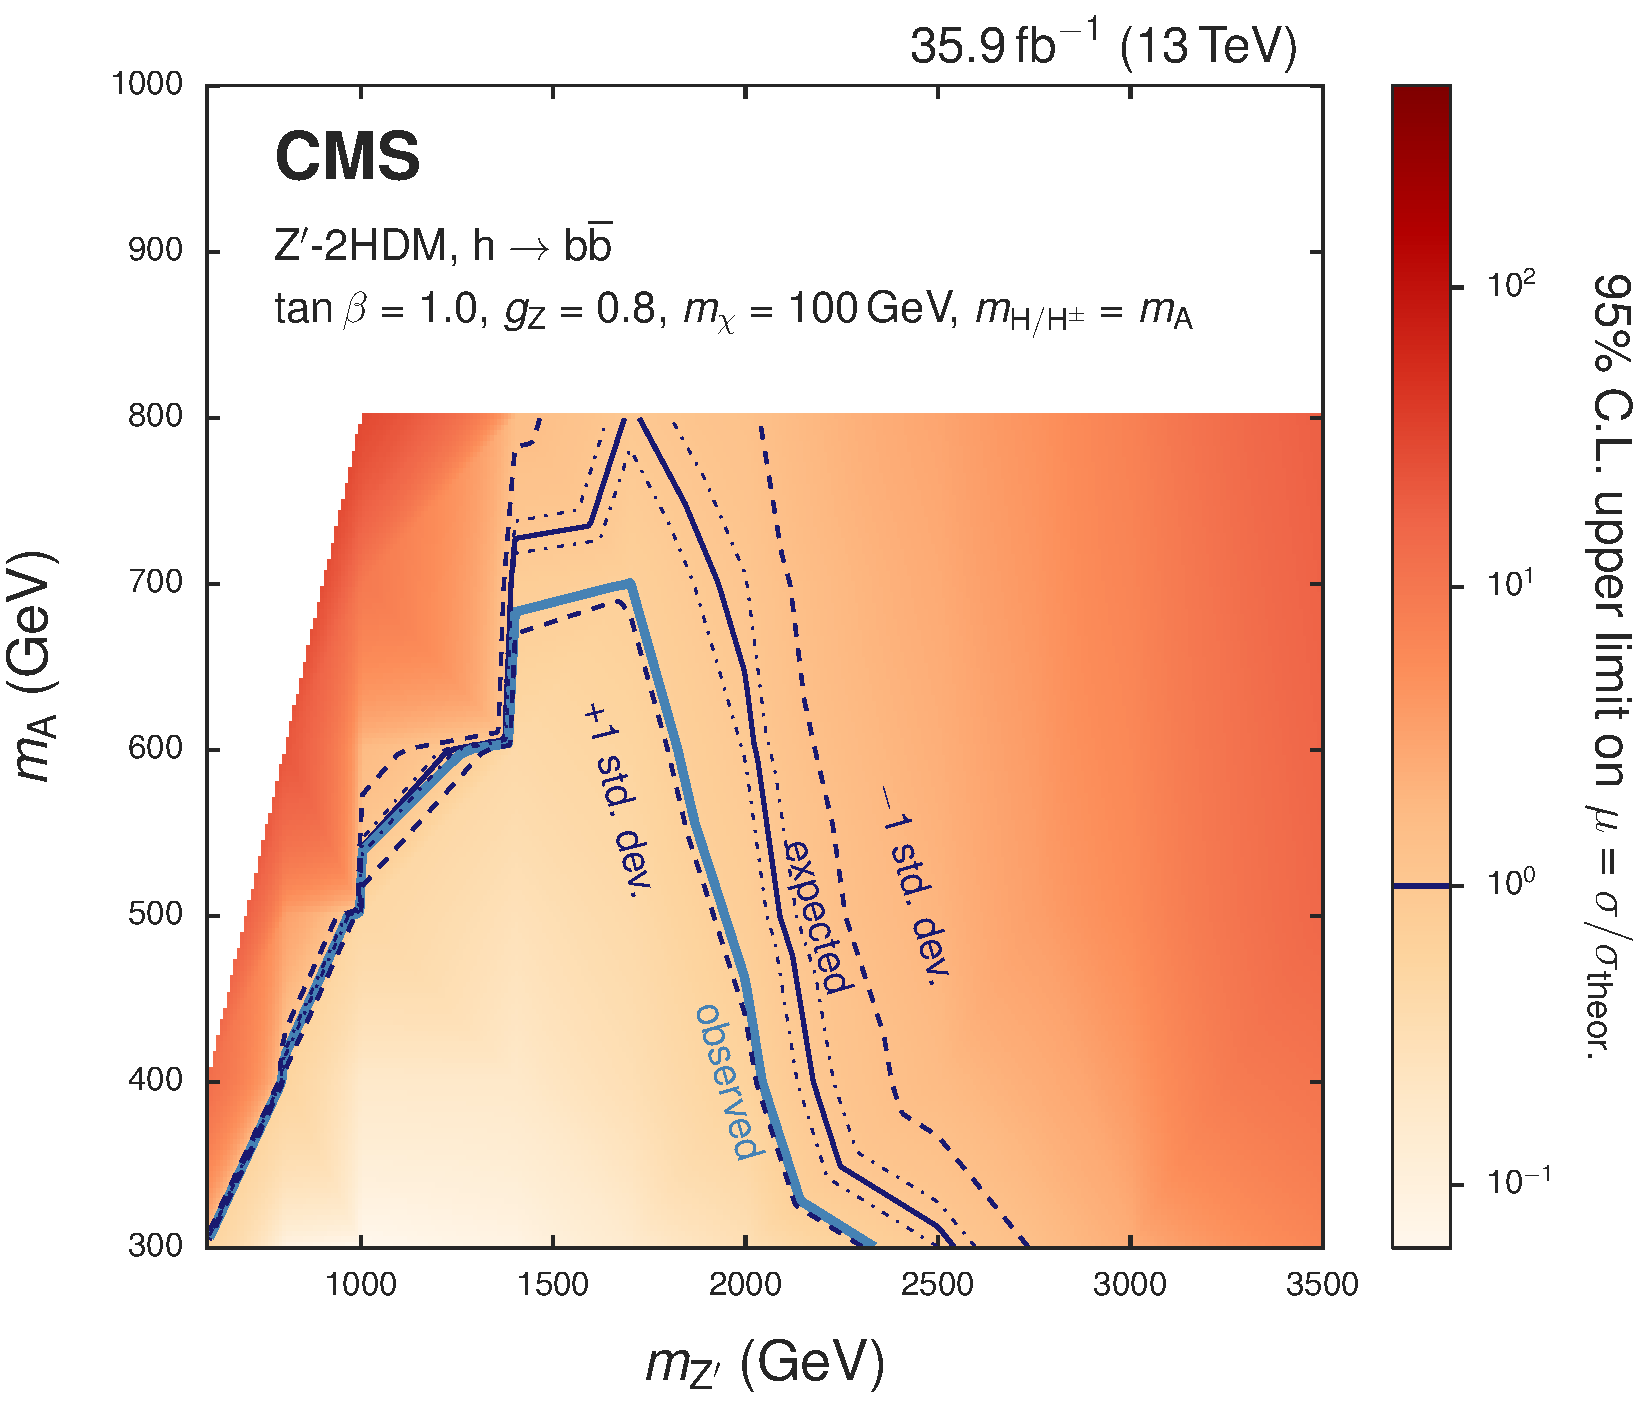
\includegraphics[width=0.475\textwidth]{figures/limits/limits_2hdm2d.png}
  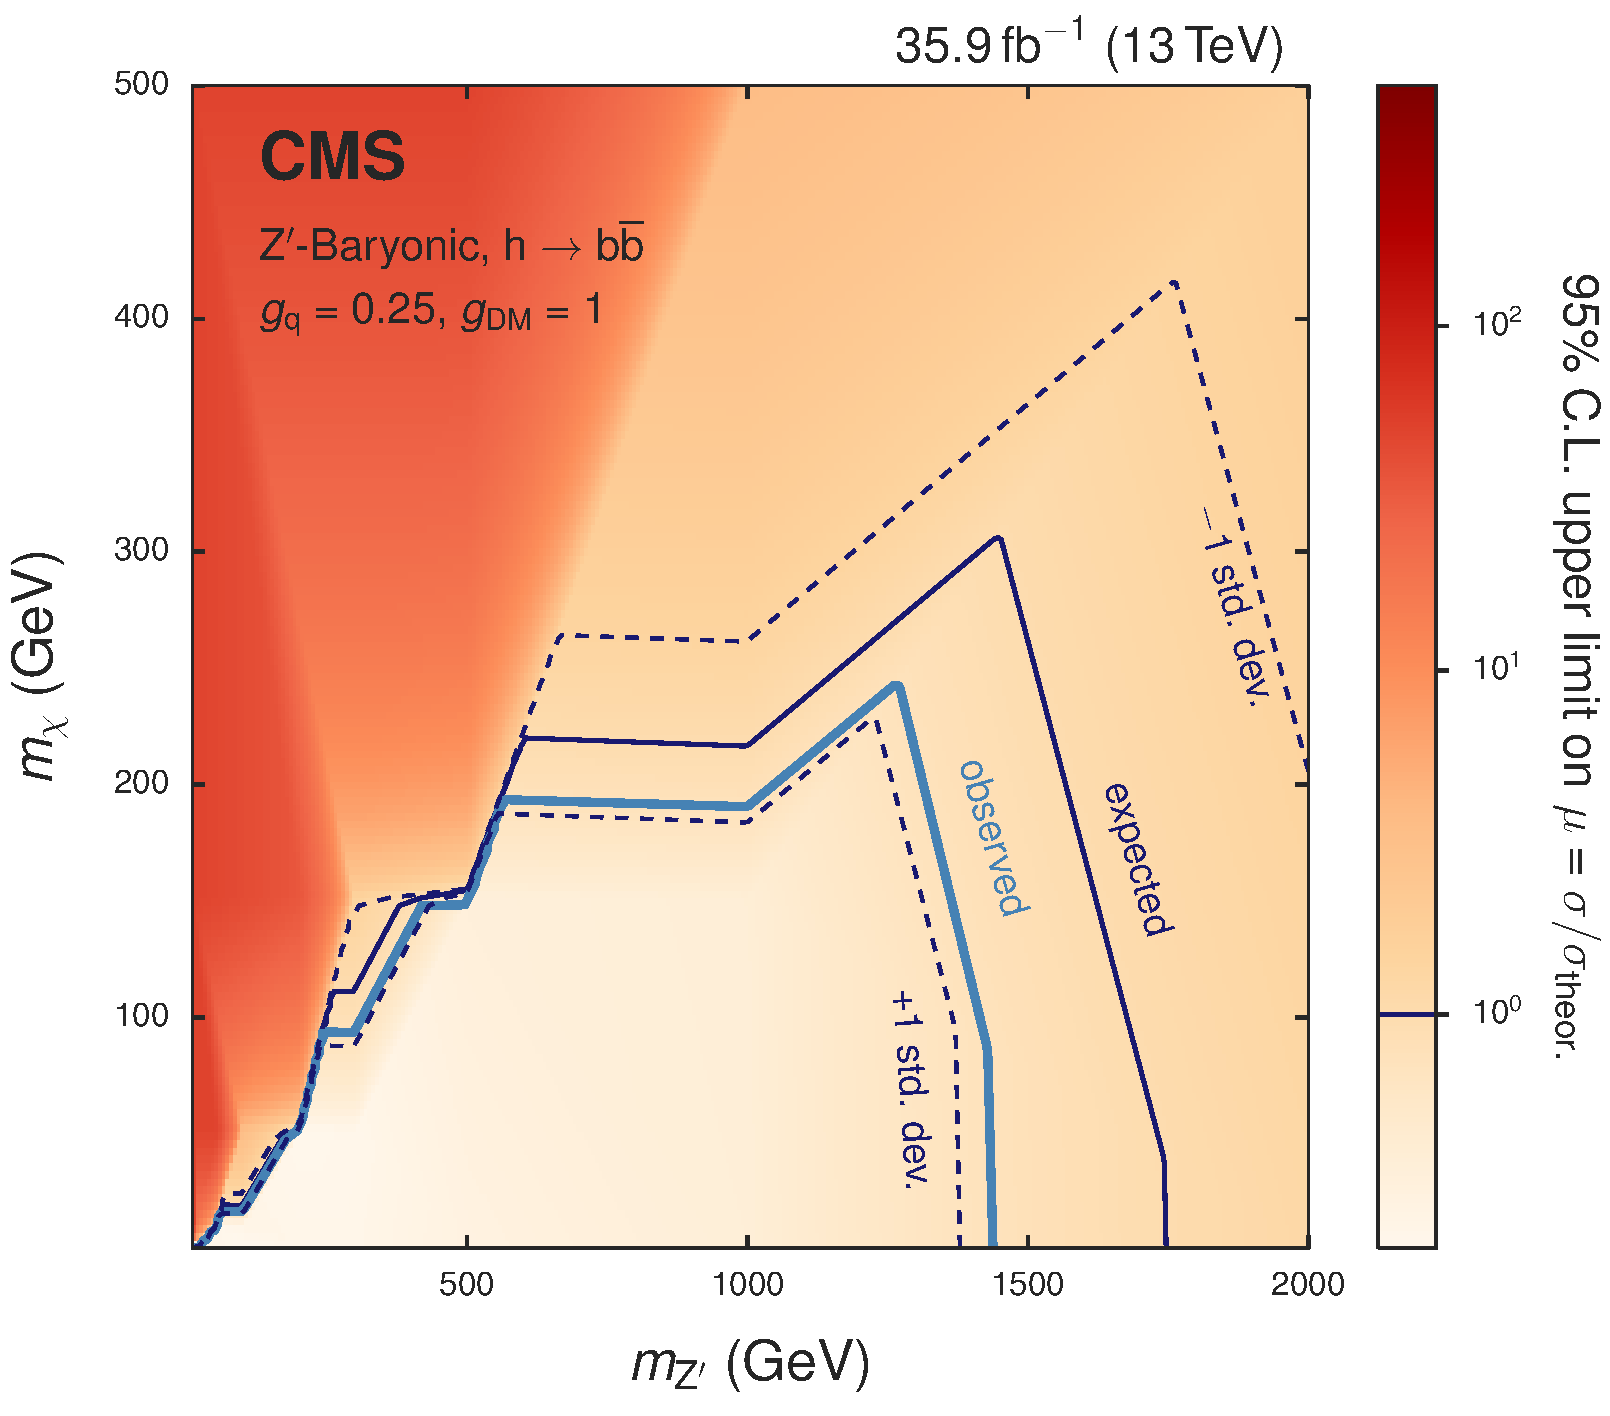
\includegraphics[width=0.475\textwidth]{figures/limits/limits_barzp2d.png}
  \caption{Upper limits on the signal strength modified for the 2HDM model (left) and Z'-Baryonic model (right).}
  \label{fig:limits}
\end{figure}

Figure~\ref{fig:limits} shows the expected and observed exclusions as a function of $m_{Z'}$ and $m_{A^0}$ for the \cPZpr-2HDM model and as a function of $m_{Z'}$ and $m_{\chi}$ for the 
baryonic $\cPZpr_{B}$ model. The excluded mass for $\mathrm{Z}'$ for $m_{A^0}=300$\,GeV is ???, while the largest excluded $\mathrm{Z}'$ mass in the $\mathrm{Z}'$-Baryonic model is ???. %Other assumptions are on $tan\beta = 1.0$, $g_{Z'} = 0.8$, and $m_{\chi} = 100$ GeV for the 2HDM, while for the Baryonic Z' model coupligs are assumed to be $g_{q} = 0.25, g_{\chi}=1~GeV$.

Results on the associated production of DM particles with Higgs boson decaying in a b-quark pair have been presented. Limits on the production cross section predicted by the \cPZpr-2HDM and the baryonic $\cPZpr_{B}$ model are set and they constitute the most stringent limits on the parameters in these models so far. 



%% **DO NOT REMOVE BIBLIOGRAPHY**
\bibliography{auto_generated}   % will be created by the tdr script.

%% examples of appendices. **DO NOT PUT \end{document} at the end
%\clearpage
\appendix
